% =============================================================
%  LES NŒUDS SCOUTS — Images Wikimedia Commons (CC BY-SA)
% =============================================================
\songsectionpage{LES NŒUDS}

\thispagestyle{empty}
\markboth{LES NŒUDS}{LES NŒUDS}

\vspace*{-4mm}

% ── NŒUD PLAT ────────────────────────────────────────────────
\noindent
\begin{minipage}[t]{0.47\textwidth}
\begin{center}
{\bfseries\sffamily Nœud plat}\\[2mm]
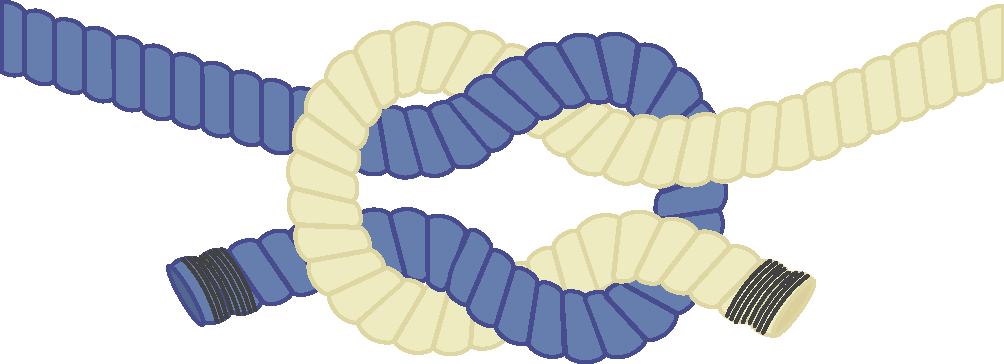
\includegraphics[height=38mm]{images/noeuds/noeud_plat.pdf}
\end{center}
\vspace{1mm}
{\small Relier deux cordes de même diamètre.}
\end{minipage}
\hfill
% ── BRÊLAGE CARRÉ ────────────────────────────────────────────
\begin{minipage}[t]{0.47\textwidth}
\begin{center}
{\bfseries\sffamily Brêlage carré}\\[2mm]
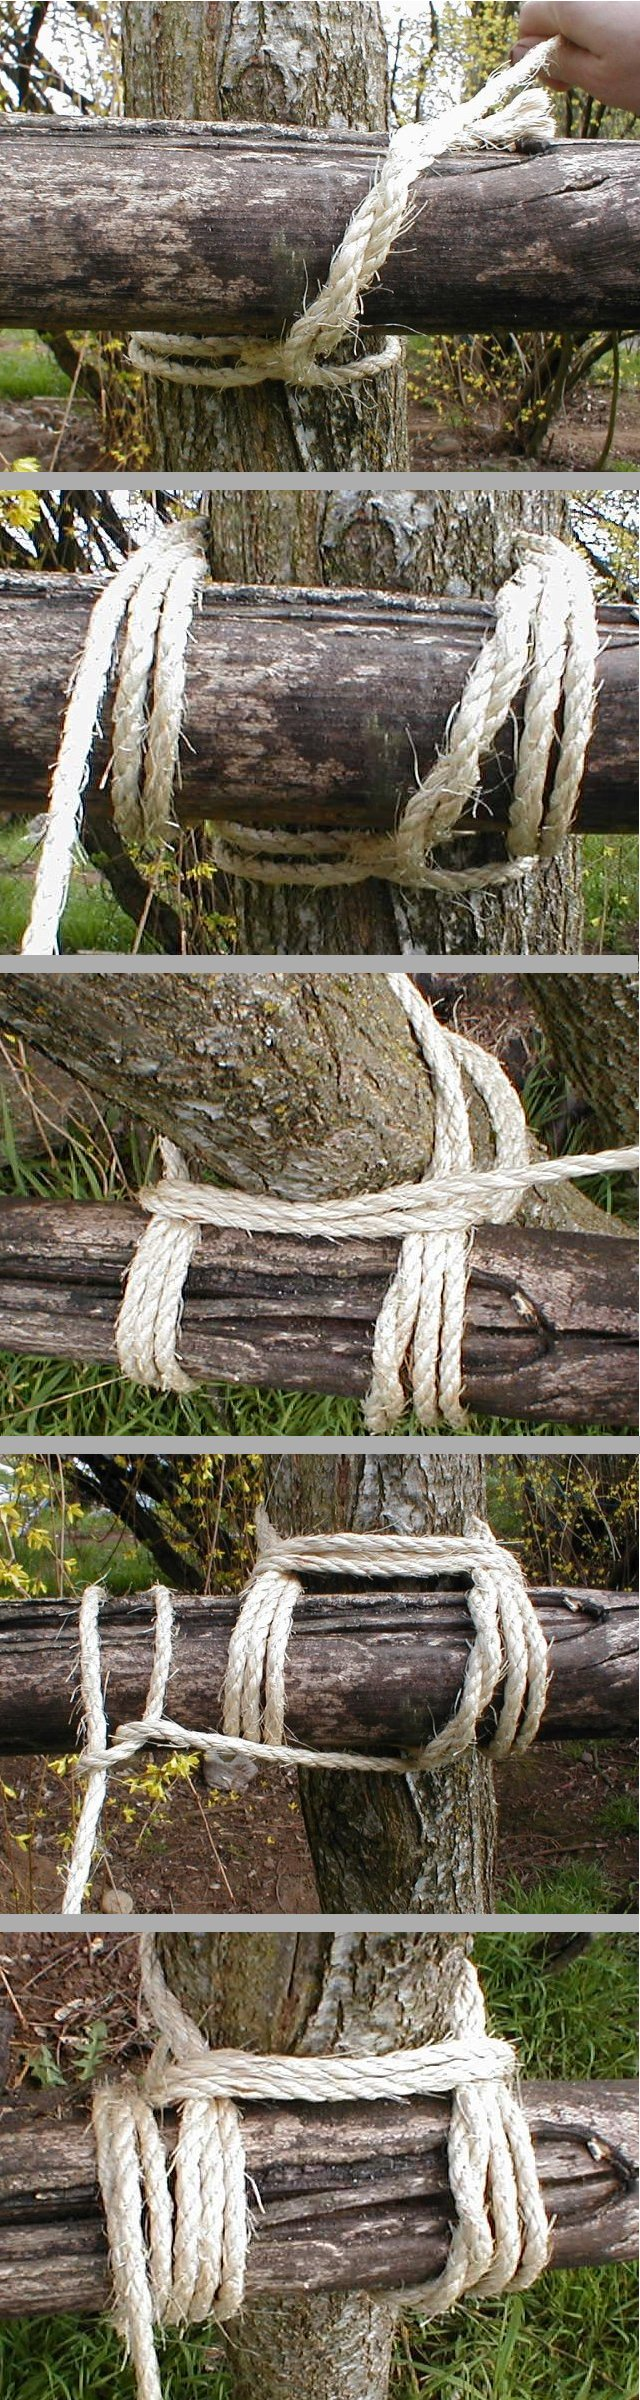
\includegraphics[height=38mm]{images/noeuds/brelage_carre.jpg}
\end{center}
\vspace{1mm}
{\small Assembler deux bâtons perpendiculaires.}
\end{minipage}

\vspace{6mm}

% ── NŒUD DE CABESTAN ─────────────────────────────────────────
\noindent
\begin{minipage}[t]{0.47\textwidth}
\begin{center}
{\bfseries\sffamily Nœud de cabestan}\\[2mm]
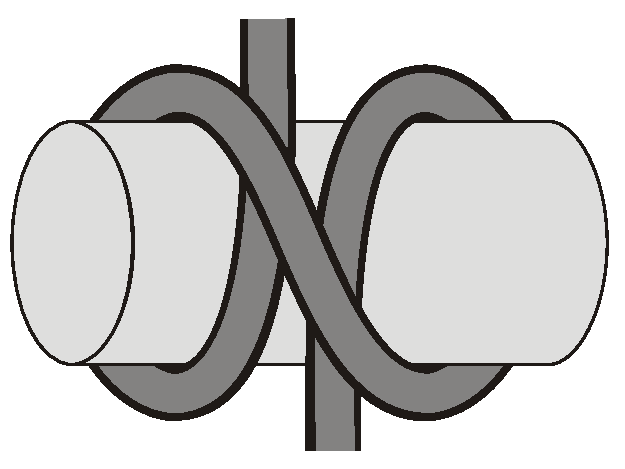
\includegraphics[height=38mm]{images/noeuds/noeud_cabestan.pdf}
\end{center}
\vspace{1mm}
{\small Attacher une corde à un piquet.}
\end{minipage}
\hfill
% ── NŒUD DE CHAISE ───────────────────────────────────────────
\begin{minipage}[t]{0.47\textwidth}
\begin{center}
{\bfseries\sffamily Nœud de chaise}\\[2mm]
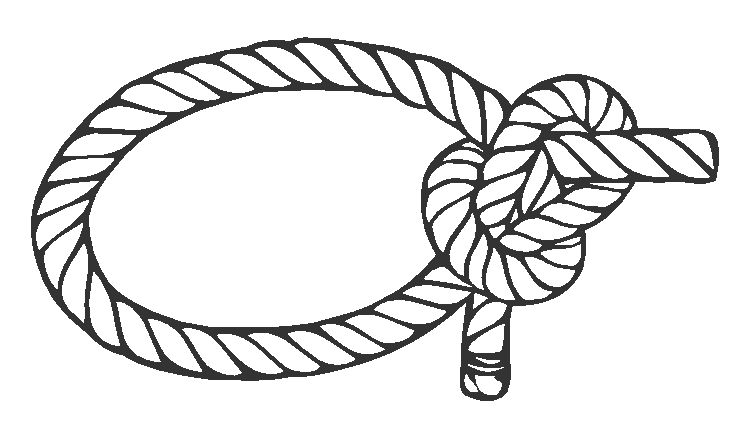
\includegraphics[height=38mm]{images/noeuds/noeud_chaise.pdf}
\end{center}
\vspace{1mm}
{\small Boucle qui ne se serre pas sous charge.}
\end{minipage}

\vfill
{\scriptsize\itshape Images : Wikimedia Commons (CC BY-SA 3.0/4.0).}

\clearpage
\thispagestyle{empty}
\markboth{LES NŒUDS}{LES NŒUDS}

\vspace*{-4mm}

% ── NŒUD DE PÊCHEUR ──────────────────────────────────────────
\noindent
\begin{minipage}[t]{0.47\textwidth}
\begin{center}
{\bfseries\sffamily Nœud de pêcheur}\\[2mm]
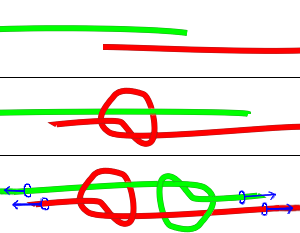
\includegraphics[height=38mm]{images/noeuds/noeud_pecheur.png}
\end{center}
\vspace{1mm}
{\small Relier deux cordes de diamètres différents.}
\end{minipage}
\hfill
% ── TOUR MORT ET DEUX DEMI-CLÉS ──────────────────────────────
\begin{minipage}[t]{0.47\textwidth}
\begin{center}
{\bfseries\sffamily Tour mort et 2 demi-clés}\\[2mm]
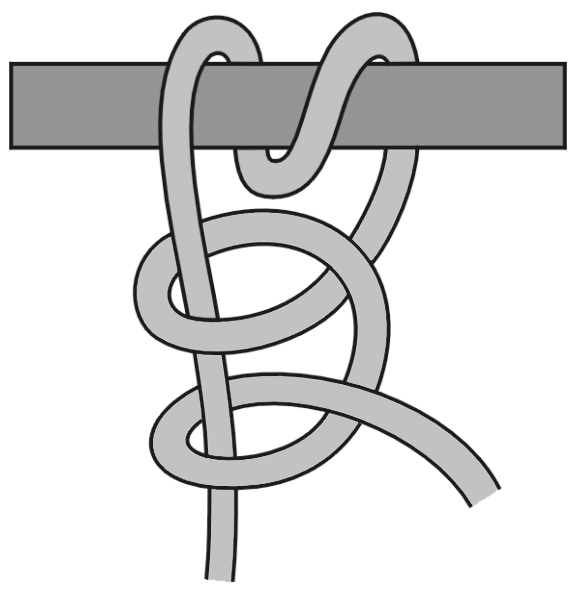
\includegraphics[height=38mm]{images/noeuds/tour_mort.png}
\end{center}
\vspace{1mm}
{\small Attacher solidement à un point fixe.}
\end{minipage}

\vspace{6mm}

% ── NŒUD EN HUIT ─────────────────────────────────────────────
\noindent
\begin{minipage}[t]{0.47\textwidth}
\begin{center}
{\bfseries\sffamily Nœud en huit}\\[2mm]
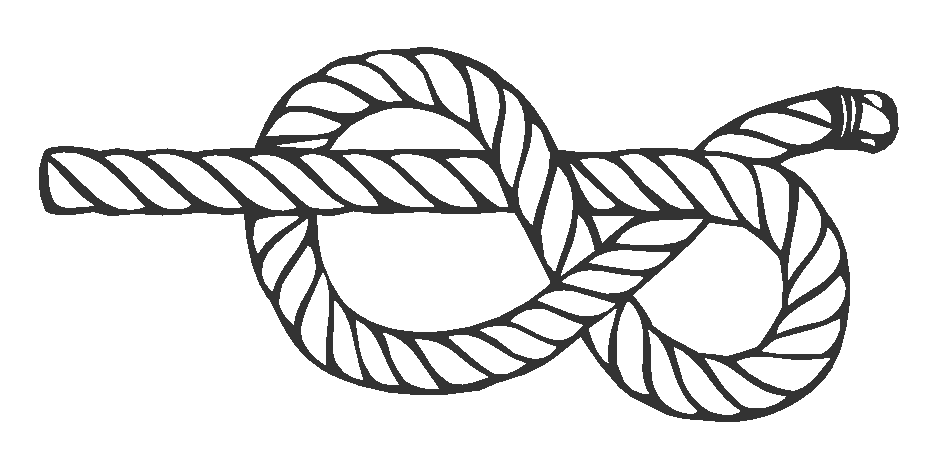
\includegraphics[height=38mm]{images/noeuds/noeud_huit.pdf}
\end{center}
\vspace{1mm}
{\small Nœud d'arrêt en bout de corde.}
\end{minipage}
\hfill
% ── TÊTE D'ALOUETTE ──────────────────────────────────────────
\begin{minipage}[t]{0.47\textwidth}
\begin{center}
{\bfseries\sffamily Tête d'alouette}\\[2mm]
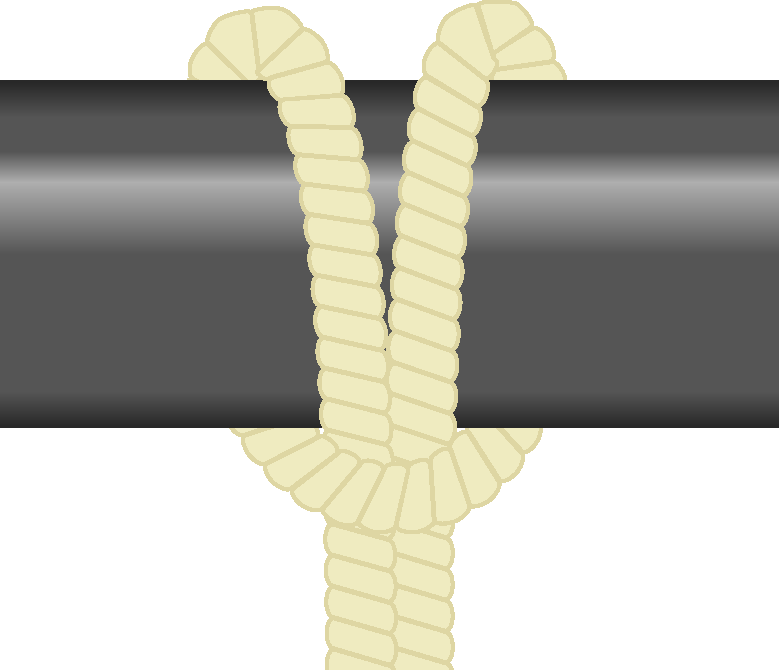
\includegraphics[height=38mm]{images/noeuds/tete_alouette.pdf}
\end{center}
\vspace{1mm}
{\small Attacher une boucle à un support.}
\end{minipage}

\vfill
{\scriptsize\itshape Images : Wikimedia Commons (CC BY-SA 3.0/4.0).}
